\subsection{Retrieving Model Equations -- NPZ Case Study}

Analysis of the NPZ validation study revealed that while AIME did not perfectly recover the original model equations after 60 generations, it achieved substantial success in reproducing key ecological mechanisms in its best-performing models. The top models achieved objective values as low as 0.0883 (lower is better) while maintaining high ecological accuracy scores (maximum total score of 7.75 out of 8; higher is better), demonstrating remarkable accuracy in reproducing NPZ dynamics. These best performers showed particularly strong recovery of phytoplankton growth dynamics and zooplankton equations (scores up to 1.0 for both; where 1.0 reflects perfect recovery of underlying dynamics), demonstrating the framework's ability to rediscover fundamental ecological relationships. However, even the best models struggled to recover nutrient mixing terms (maximum score of 0 - indicating this mechanism was never suggested in any capacity), suggesting some ecological mechanisms were more challenging to identify from time-series data alone.

\begin{figure}[H]
\centering
\includegraphics[width=\textwidth]{../Figures/NPZ_combined}
\caption{Evolution and performance of the best NPZ model. (A) Training progress showing the objective value across generations on a log-scale. (B) Time series comparison between ground-truth and modelled NPZ dynamics for the best-performing model (objective value = 0.0883). The plots show the temporal evolution of nutrient, phytoplankton, and zooplankton concentrations (g C m\textsuperscript{-3}). Blue solid lines represent ground-truth data, while orange dashed lines show model predictions, demonstrating the model's ability to capture key ecological patterns and phase relationships between trophic levels.}
\label{fig:npz_timeseries}
\end{figure}

Importantly, we found negative correlations between objective values and ecological accuracy scores, indicating that improvements in model fit were generally achieved through ecologically sound mechanisms rather than overfitting. The strongest correlation was observed for phytoplankton growth equations (r = -0.461, p = 0.002), followed by nutrient uptake (r = -0.399, p = 0.008). The total ecological score also showed a significant negative correlation with objective values (r = -0.380, p = 0.012), suggesting that models achieving better fits tended to incorporate more correct ecological mechanisms.

The best-performing models achieved objective values as low as 0.112, demonstrating strong predictive accuracy while maintaining meaningful ecological structure. A detailed analysis of individual ecological characteristics (see Figure~\ref{fig:ecological_characteristics} in Supplementary Materials) revealed that some mechanisms were more readily recovered than others.

\begin{figure}[H]
\centering
\includegraphics[width=1.0\textwidth]{../Figures/ecological_vs_objective_total}
\caption{Log-log Relationship between total ecological accuracy score and model performance (objective value). Lower objective values indicate better model fit, while higher ecological scores indicate closer alignment with known NPZ model mechanisms. The data distribution appears to cluster into two groups -- models with total ecological scores above 6 and those below 6 -- suggesting a potential threshold effect where certain key ecological mechanisms significantly improve model performance. This pattern may be driven by specific equation terms that, once correctly implemented, substantially enhance model accuracy.}
\label{fig:ecological_total}
\end{figure}

\subsection{COTS Case Study}
\label{sec:cots_data}
For all but one LLM, AIME was able to generate ecosystem models with prediction accuracy that was approaching the quantitative fit of the expert-developed model (objective value (NMSE): 0.2312). After ten generations, objective values across LLMs were as follows: gpt4.1 achieved the best objective value (0.3488; which was achieved in the first generation and unimproved over subsequent generations), followed by Claude Sonnet-3.7 (0.5204), then o3-mini (0.5606), o4-mini (0.5786), and finally Claude Sonnet-3.6 (0.6599). Surprisingly, despite high scores on common benchmarks, Google's Gemini-2.5-pro was not able to produce a single numerically stable model after five generations, and thus we terminated its process. Component-specific analysis revealed varying levels of prediction accuracy, with models showing strongest performance in predicting fast-growing coral cover and slow-growing coral cover, while maintaining reasonable accuracy for the more volatile COTS abundance patterns (Figure \ref{fig:llm_comparison}).

The ecological models produced by AIME exhibited substantial structural diversity in their ecological mechanisms and usability, while sharing several foundational elements. Across all models, density-dependent COTS population growth, resource limitation based on coral availability, and differential impacts on fast versus slow-growing coral species emerged as common features.

Temperature effects were implemented through markedly different approaches across the LLMs. Claude 3.6 and Claude 3.7 Sonnet employed Gaussian response curves where COTS survival peaks at optimal temperatures. In contrast, the o3-mini and gpt 4.1 models utilized linear temperature factors that directly modify growth rates. The o4-mini model took yet another approach, incorporating a number of abstract and vague parameters such as 'environemtal modifier' and explicit outbreak parameters without explicitly modelling temperature.

The representation of COTS-coral interactions similarly varied across models. The o3 mini LLM implemented resource limitation with quadratic adjustment factors for outbreak triggering, creating non-linear responses to coral availability. Claude 3.6 Sonnet featured temperature-dependent recruitment with resource limitation based on total coral cover. Claude 3.7 Sonnet employed Holling Type II functional responses for predation with explicit food limitation effects that increase COTS mortality when coral cover is low. The o4 mini model utilized resource limitation with saturating functions and quadratic terms to capture diminishing returns in resource uptake. Finally, the gpt 4.1 model incorporated differential predation on coral types with varying assimilation efficiencies.

There were notable differences in the behaviour and speed of convergence for all of the LLMs we tested Figure \ref{sec:convergence}. The o3-mini model completed ten generations in as little as 41 minutes. The two Claude-Sonnet LLMs and OpenAI's GPT4.1 were able to generate well-functioning models in a single generation, but struggled to improve upon previous generations, whereas o3-mini and o4-mini (the two `reasoning' models we included in this study) were able to consistently improve upon previous generations. Due to this behaviour, we decided to run o4-mini for an additional 90 generations (100 generations total), to see if it would converge at or near the human model. Ultimately, it reached an objective value of 0.3486, but was unable to fully capture the outbreak dynamics of the CoTS as requested in the research topic (Figure \ref{fig:llm_comparison}). We note that, for the purposes of this initial exploration, the objective function was weighted equally for all time-series, whereas the human modeller may have prioritised capturing the two outbreaks exhibited in the COTS time-series. 

\begin{figure}[H]
    \centering
    \includegraphics[width=1.0\textwidth]{../Figures/llm_predictions_comparison.png}
    \caption{Comparison of model predictions across ecosystem components. The plots show observed versus predicted values for COTS abundance, fast-growing coral cover, and slow-growing coral cover, demonstrating the models' ability to capture key ecological patterns and relationships. Objective values (obj) shown in the legend represent the normalised mean squared error for all three variables, where lower values indicate better model performance. NB: Gemini-2.5-pro is not shown as it failed to produce a numerically stable model.}
    \label{fig:llm_comparison}
    \end{figure}
    

\subsubsection{Time-Series Prediction Performance}

Because the o4-mini LLM demonstrated a high capability to improve quantitative performance across generations, we used it as the base LLM to test whether the AIME framework could create models that are capable of predicting out of sample datapoints. After ten generations, we found that the best performing model (objective value: 0.4677) had a reasonable degree of out-of-sample predictions performance on the withheld test dataset, with particularly strong predictive power for fast-growing coral cover (R² = 0.768, RMSE = 2.169, MAE = 2.025). 

For slow-growing coral cover, the model achieved moderate predictive accuracy (R² = 0.187, RMSE = 1.929, MAE = 1.568), effectively capturing the general declining trend while showing some deviation in precise values. COTS population predictions demonstrated reasonable accuracy (R² value 0.569, RMSE = 0.073, MAE = 0.064) despite not fully capturing the magnitude of peaks in COTS abundance in the training data.

Figure~\ref{fig:validation_combined} illustrates these prediction capabilities, showing both training period performance (pre-1997) and out-of-sample predictions (1997-2005). Interestingly, in contrast to the o4-mini's fairly vague equations described above, this iteration featured more tangible parameter and equations formulations (See model details in Section \ref{sec:best_out_of_sample}). The model's ability to maintain consistent error metrics (RMSE and MAE) while capturing both rapid population dynamics and slower coral cover changes suggests it has successfully identified fundamental ecological relationships governing this system.


\begin{figure}[H]
\centering
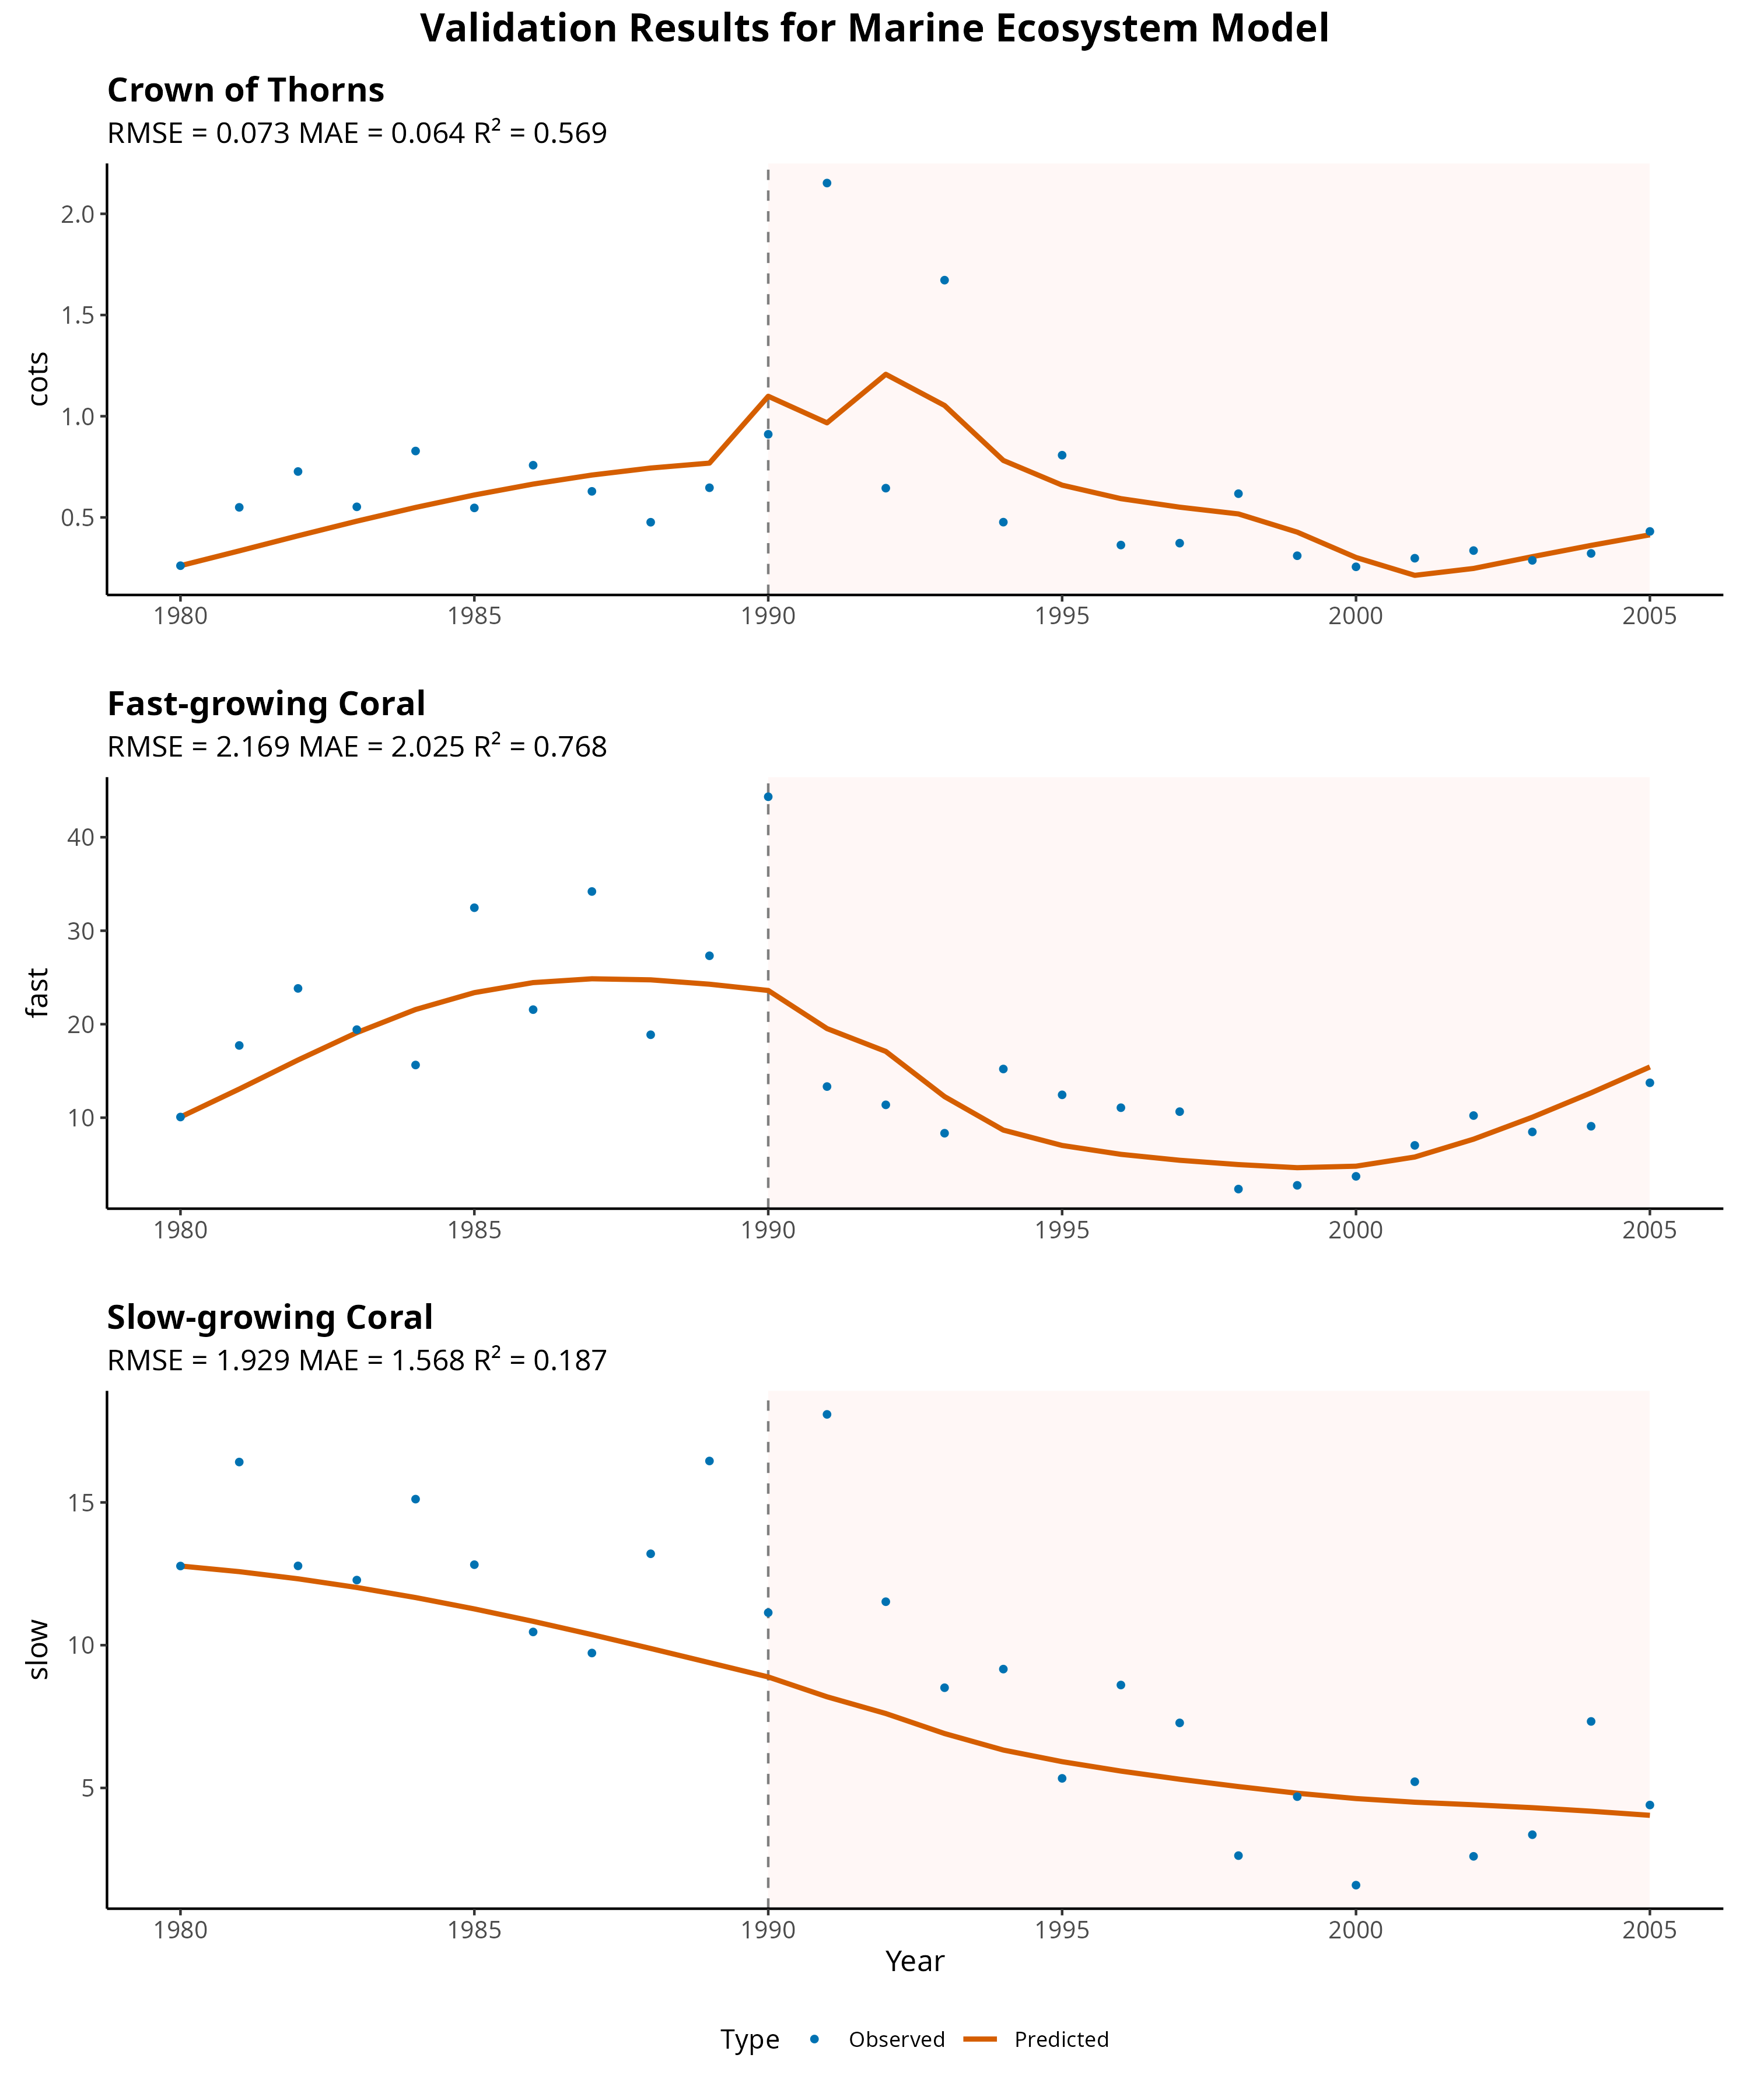
\includegraphics[width=1.0\textwidth]{../Figures/combined_validation.png}
\caption{Time-series validation of the best-performing AI model (GPT 4.1) showing predictions against observed data. The model was trained on 70\% of the time-series data (pink shaded region) and validated on the remaining unseen 30\% of the time-series data (white region). Top: COTS abundance predictions showing some capture of population variability. Middle: Fast-growing coral cover predictions demonstrating tracking of recovering . Bottom: Slow-growing coral cover predictions illustrating strong capture of recovery dynamics. Orange lines represent model predictions, blue dots show observed data.}
\label{fig:validation_combined}
\end{figure}
